\documentclass[10pt]{beamer}
\usetheme{Warsaw}
\title{Oh-My-Git}
\author{Ashik Salman}
\institute[UMBC]{Awesome Git tweaks \\
  ..... \\
  Backend Developer \\
  Chillr, Backwater Technologies \\
  Kochi, Kerala \\

}
\date{September 25, 2016}
\begin{document}

%----Title----%

\begin{frame}[plain]
  \titlepage
\end{frame}
	
%----Slides----%
%-1-%
\begin{frame}
  \begin{center}
    \Huge{oh-my-git, what?}
  \end{center}
\end{frame}

%-2-%
\begin{frame}
	\frametitle{Generic View}
	\textbf{Git Tool}
	\begin{center}
	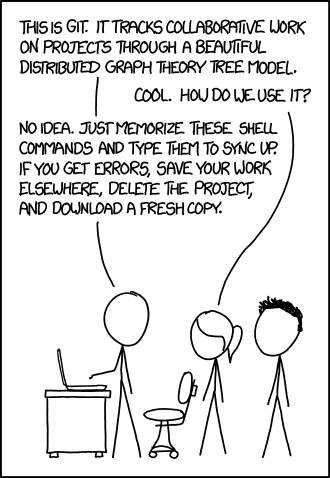
\includegraphics[width=0.42\textwidth]{git-xkcd.png}
	\end{center}
\end{frame}

%-3-%
\begin{frame}
  \begin{center}
    \Huge{Versioning by Patch changes}
  \end{center}
\end{frame}

%-4-%
\begin{frame}[fragile]
  \frametitle{Git with Patches}
  \begin{block}{Add changes by patches}
    \begin{verbatim}
      $ git add -p
      $ git add -i (interactive menu)
    \end{verbatim}
  \end{block}
  \pause
  \begin{block}{Checkout changes by patches(Remove un-staged changes)}
    \begin{verbatim}
      $ git checkout -p
    \end{verbatim}
  \end{block}
  \pause
  \begin{block}{Reset changes by patches(Remove staged changes)}
    \begin{verbatim}
      $ git reset -p
    \end{verbatim}
  \end{block}
\end{frame}

%-5-%
\begin{frame}
  \frametitle{oh-my-git !!!}
  \begin{alertblock}{Scenario 1}
    I did something terribly wrong, I want to got to a stage where everything worked fine.
  \end{alertblock}
  \pause
  \begin{block}{Why... ?}
    You can use this to get back stuff you accidentally deleted, or just to remove some stuff you
    tried that broke the repo, or to recover after a bad merge, or just to go back to a time when things actually worked.
  \end{block}
\end{frame}

%-6-%
\begin{frame}[fragile]
  \frametitle{oh-my-git !!!}
  \begin{example}[Solution]
    \begin{verbatim}
      $ git reflog
      # you will see a list of every thing you've done in git, across all branches!
      # each one has an index HEAD@{index}
      # find the one before you broke everything
      $ git reset HEAD@{index}
    \end{verbatim}
  \end{example}
  \pause
  \begin{block}{Note !}
    If the work was committed at any point, then it can be recovered from the reflog.
    By default all commits stay alive in the reflog for at least 2 weeks.
  \end{block}
\end{frame}

%-7-%
\begin{frame}
  \frametitle{oh-my-git !!!}
  \begin{alertblock}{Scenario 2}
    I just committed some changes and immediately realized I need to make one small change.
  \end{alertblock}
\end{frame}

%-8-%
\begin{frame}[fragile]
  \frametitle{oh-my-git !!!}
  \begin{example}[Solution]
    \begin{verbatim}
      # make your change
      $ git add .  # or add individual files
      $ git commit --amend
      # follow prompts to change or keep the commit message
      # now your last commit contains that change!
    \end{verbatim}
  \end{example}
  \pause
  \begin{block}{Note !}
    You could also make the change as a new commit and then do rebase -i in order to squash them both together,
    but this is about a million times faster.
  \end{block}
\end{frame}

%-9-%
\begin{frame}
  \frametitle{oh-my-git !!!}
  \begin{alertblock}{Scenario 3}
   I accidentally committed something to master that should have been on a brand new branch!
  \end{alertblock}
\end{frame}

%-10-%
\begin{frame}[fragile]
  \frametitle{oh-my-git !!!}
  \begin{example}[Solution]
    \begin{verbatim}
      # create a new branch from the current state of master
      $ git branch some-new-branch-name
      # remove the commit from the master branch
      $ git reset HEAD~ --hard
      $ git checkout some-new-branch-name
      # your commit lives in this branch now :)
    \end{verbatim}
  \end{example}
  \pause
  \begin{block}{Note !}
    This doesn't work if you've already pushed to origin, and if you tried other things first,
    you might need to git reset HEAD@{number} instead of HEAD~.
  \end{block}
\end{frame}

%-x-%
\begin{frame}
  \begin{center}
    \Huge{Git Merge (Conflicts!!!)}
  \end{center}
\end{frame}

%-x-%
\begin{frame}
  \begin{center}
    \Huge{Git rebase - interactive (Conflicts !!!)}
  \end{center}
\end{frame}

%-x-%
\begin{frame}
  \begin{center}
    \Huge{Git Stash - Easy work save/restore }
  \end{center}
\end{frame}

%-x-%
\begin{frame}
  \begin{center}
    \Huge{Thank You}
  \end{center}
\end{frame}

%-x-%
\begin{frame}
	\frametitle{Questions?}
	\begin{center}
	
\includegraphics[width=0.35\textwidth]{q5.jpg}
	\end{center}
\end{frame}

%----Slides----%

\end{document}
